\documentclass[12pt,a4paper]{article}
\usepackage[utf8]{}
\usepackage{amsmath}
\usepackage{amsfonts}
\usepackage{xcolor}
\usepackage{titlesec}
\usepackage{mdframed}
\usepackage[english]{babel}
\usepackage{amssymb}
\usepackage{pgf,tikz,pgfplots}
\usepackage{graphicx}
\graphicspath{ {figures/} }
\usepackage{array}
\usepackage{cases}
\usepackage{listings}
\usepackage{color}
\usepackage{float} 
\usepackage{hyperref}
%\usepackage{minitoc}
\pgfplotsset{compat=1.5}
\usepackage{mathrsfs}
\usetikzlibrary{arrows, calc}
\usepackage{fancyhdr}
\pagestyle{fancy}
\usepackage[labelsep=endash]{caption}
\pagestyle{empty}
\definecolor{dkgreen}{rgb}{0,0.6,0}
\definecolor{gray}{rgb}{0.5,0.5,0.5}
\definecolor{mauve}{rgb}{0.58,0,0.82}
\lstset{frame=tb,
  language=C++,
  aboveskip=3mm,
  belowskip=3mm,
  showstringspaces=false,
  columns=flexible,
  basicstyle={\small\ttfamily},
  numbers=none,
  numberstyle=\tiny\color{gray},
  keywordstyle=\color{blue},
  commentstyle=\color{dkgreen},
  stringstyle=\color{mauve},
  breaklines=true,
  breakatwhitespace=true,
  tabsize=3
}
\renewcommand{\listfigurename}{Figures}
\renewcommand{\listtablename}{Tables}
\newcommand{\tabitem}{~~\llap{\textbullet}~~}
\usepackage[left=2cm,right=2cm,top=2cm,bottom=2cm]{geometry}
\author{Nguyễn Văn Lộc}
\newmdenv[linecolor=black,skipabove=\topsep,skipbelow=\topsep,
leftmargin=-5pt,rightmargin=-5pt,
innerleftmargin=5pt,innerrightmargin=5pt]{mybox}
\begin{document}
\fancyhf{}
\lhead{Lab 3: Sorting}
\chead{}
\rhead{20120131 - Nguyen Van Loc}
\cfoot{\thepage}
\rfoot{}
\lfoot{}
\pagestyle{fancy}
\renewcommand{\headrulewidth}{0pt}
\renewcommand{\footrulewidth}{0pt}
\begin{titlepage}
\begin{mybox}
\begin{center}
\fontsize{12}{12}\selectfont
\textbf{VIETNAM NATIONAL UNIVERSITY HO CHI MINH CITY}\\
\textbf{UNIVERSITY OF SCIENCE}\\
\textbf{FACULTY OF INFORMATION TECHNOLOGY}
\end{center}
\vskip 2 cm
\begin{figure}[H]
\begin{center}

\includegraphics[scale=0.25]{logo}
\end{center}
\end{figure}
\vskip 2 cm
\begin{center}
\fontsize{18}{14}\selectfont
\textbf{REPORT FOR LAB 3: SORTING}\\
\vskip 0.5 cm
\fontsize{20}{16}\selectfont
\textbf{DATA STRUCTURES AND ALGORITHMS}\\
\vskip 0.5 cm
\fontsize{18}{12}\selectfont
\textbf{TOPIC: SORTING ALGORITHMS}
\end{center}
\vskip 2 cm
\fontsize{14}{12}\selectfont
\textbf{Instructor:} Master Bui Huy Thong\\
\textbf{Class:} 20CTT1TN\\
\textbf{Student:} 20120131 \(-\) Nguyen Van Loc
\vskip 4 cm
\begin{center}
\textbf{HO CHI MINH CITY, NOVEMBER 2021}
\end{center}
\end{mybox}
\end{titlepage}
\section{Information page}
\textbf{Name:} Nguyen Van Loc\\
\textbf{Student ID:} 20120131\\
\textbf{Class:} 20CTT1TN\\
\textbf{Subject:} Data structures and algorithms\\
\textbf{Lecturer:} Doctor Nguyen Thanh Phuong\\
\textbf{Instructor:} Master Bui Huy Thong\\
\textbf{Topic:} Sorting algorithms

\newpage

\section{Introduction page}
I have completed 11/11 required algorithms, including: selection sort, insertion sort, bubble sort, shaker sort, shell sort, heap sort, merge sort, quick sort, counting sort, radix sort, and flash sort\\
For output specifications, I have completed 5/5 commands, 3 for algorithm mode and 2 for comparison mode.\\
Below is the hardware specifications of the computer I used to run these algorithms:
\begin{figure}[H]
\begin{center}
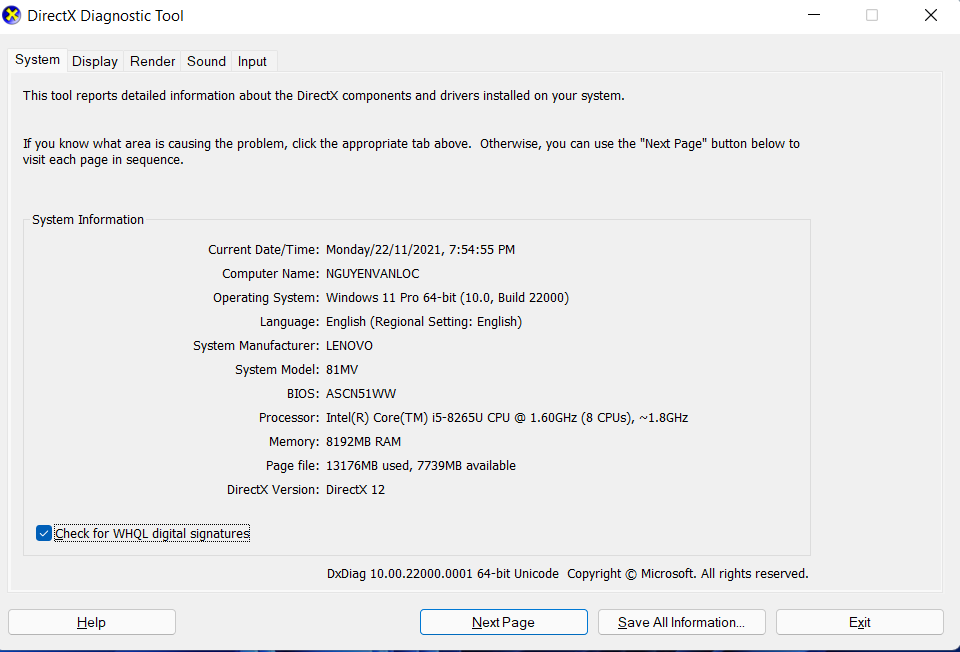
\includegraphics[scale=0.75]{hardware}
\end{center}
\caption{Hardware specifications}
\end{figure}

\newpage

\tableofcontents

\listoffigures
\listoftables

\newpage

\section{Algorithm presentation}
In this section, I will present the algorithms implemented in the project: ideas, step-by-step descriptions, and complexity evaluations. Varians/improvements of an algorithm, if there is any, will be also mentioned.\\
In this project, sorting algorithms are only used to sort the array in ascending order. Sorting in descending order will be similar.\\
Most of pseudocodes in this section will be presented in Pascal, with the 1-base array.
\subsection{Selection sort}
Selection sort is one of the simplest sorting algorithms.\\
Basic ideas of this algorithm is as followed:
\begin{itemize}
	\item In the first turn, choose  the minimum element in a[1..n], then swap it with a[1], that means a[1] becomes the minimum element of the array.
	\item In the second turn, choose the minimum element in a[2..n], then swap it with a[2], so that a[2] becomes the second lowest element of the array.
	\item ...
	\item In the i-th turn, choose the minimum in a[i..n], then swap it with a[i].
	\item In the (n-1)-th turn, choose the lower between a[n - 1] and a[n], then swap it with a[n-1].
\end{itemize}
\textbf{Pseudocodes}: \cite{gtvlt}
\lstset{language=Pascal} 
\begin{lstlisting}
begin
	for i := 1 to  n - 1 do
	begin
		jmin := i;
		for j := i + 1 to n do
			if (a[j] < a[jmin]) then jmin := j;
		if (jmin != i) then swap(a[jmin], a[i]);
	end
end
\end{lstlisting}
\textbf{Time complexity:} \cite{sscomp}
\begin{itemize}
\item Worst case: $O \left( {n^2} \right).$
\item Best case: $O \left( {n^2} \right).$
\item Average case: $O \left( {n^2} \right).$
\end{itemize}
\textbf{Space complexity:} $O \left( 1 \right).$ \cite{sscomp}

\subsection{Insertion sort}
\textbf{Ideas:} Consider the array a[1..n].\\
We see that the subarray with only one element a[1] can be seen as sorted.\\
Consider a[2], we compare it with a[1], if a[2] < a[1], we insert it before a[1].\\
With a[3], we compare it with the sorted subarray a[1..2], find the position to insert a[3] to that subarray to have an ascending order.\\
In a general speech, we will sort the array a[1..k] if the array a[1..k - 1] is already sorted by inserting a[k] to the appopriate position.\\
\textbf{Pseudocodes}: \cite{gtvlt}
\lstset{language=Pascal} 
\begin{lstlisting}
begin
	for i := 2 to n do
		begin
		temp := a[i];
		j := i - 1;
		while (j > 0) and (temp < a[j]) do
			begin
			a[j + 1] = a[j];
			dec(j);
			end
		a[j + 1] = temp;
		end
end
\end{lstlisting}
\textbf{Time complexity: } \cite{comp}
\begin{itemize}
\item Worst case: $O \left( {n^2} \right).$
\item Best case: $O \left( {n} \right),$ in case the array is already sorted.
\item Average case: $O \left( {n^2} \right).$
\end{itemize}
\textbf{Space complexity:} $O \left( {1} \right).$ \cite{comp}\\
\textbf{Improvements:}
\begin{itemize}
\item Binary insertion sort $-$ find the position to insert using binary search, which reduces the number of comparisons. Details at link: \url{https://www.geeksforgeeks.org/binary-insertion-sort/}.
\item Another improvement of insertion sort is shell sort, which will be presented in section \ref{shellsort}
\end{itemize}

\subsection{Bubble sort}
\textbf{Ideas:} Bubble sort is the simples sorting algorithm, which swaps the adjacent elements if they are in wrong order, repeatedly $n$ times.\\
After the $i-$th turn, the $i-$th smallest element will be swapped to position $i.$\\
\textbf{Pseudocodes:} \cite{gtvlt}
\lstset{language=Pascal} 
\begin{lstlisting}
begin
	for i := 2 to n do
		for j := n downto i do
		if (a[j - 1] > a[j]) then swap(a[j - 1], a[j]);
end
\end{lstlisting}
\textbf{Time complexity:} $O \left( {n^2} \right),$ not mentioned how the input data is. \cite{gtvlt}\\
\textbf{Space complexity:} $O \left( {1} \right).$ \cite{comp}\\
\textbf{Variations:} There are some variations in the implementation.
\begin{itemize}
\item Instead of top-down with \lstinline{j}, we can iterate from the bottom up, from \lstinline{i + 1} to \lstinline{n}.
\item Another variation is \lstinline{j} iterates from \lstinline{1} to \lstinline{n - i}. This is the version that I choose in my project.
\end{itemize}
\textbf{Improvements:} An improvement of bubble sort is shaker sort, which we will research in section \ref{shakersort}.

\subsection{Shaker sort (Cocktail sort)}
\label{shakersort}
\textbf{Ideas:} 
Shaker sort, also called cocktail sort or bi-directional bubble sort, is an improvement of bubble sort. In bubble sort, elements are traversed from left to right, i.e. in one direction only. But shaker sort will traverse in both direction, from left to right and from right to left, alternatively. \cite{shaker}\\
\textbf{Pseudocode:} \cite{thayP}
\lstset{language=Pascal} 
\begin{lstlisting}
begin
	left := 2;
	right := n;
	k := n;
	repeat 
	for j := right downto left do
		if (a[j - 1] > a[j]) then
			begin
			swap(a[j - 1], a[j]);
			k = j;
			end
	left = k + 1; //the last swap position
	for j := left to right do
		if (a[j - 1] > a[j]) then
			begin
			swap(a[j - 1], a[j]);
			k = j;
			end
	right = k - 1;
	until left > right;
	
end
\end{lstlisting}
\textbf{Time complexity:} \cite{shaksort}
\begin{itemize}
\item Worst case: $O \left( {n^2} \right).$
\item Best case: $O \left( {n} \right),$ in case the array is already sorted.
\item Average case: $O \left( {n^2} \right).$
\end{itemize}
\textbf{Space complexity:} $O \left( {1} \right).$ \cite{shaksort}

\subsection{Shell sort}
\label{shellsort}
A drawback of insertion sort is that we always have to insert an element to a position near the beginning of the array. In that case, we use shell sort.\\
\textbf{Ideas:} Consider an array a[1..n]. For an integer $h:$ $1 \leqslant h \leqslant n,$ we can divide the array into $h$ subarrays:
\begin{itemize}
\item Subarray 1: a[1], a[1 + h], a[1 + 2h]...
\item Subarray 2: a[2], a[2 + h], a[2 + 2h]...
\item ...
\item Subarray h: a[h], a[2h], a[3h] ...
\end{itemize}
Those subarrays are called subarrays with step $h.$ With a step $h,$ shell sort will use insertion sort for independent subarrays, then similarly with $\frac{h}{2}, \frac{h}{4}, ...$ until $h = 1.$\\
\textbf{Pseudocodes:}
\lstset{language=Pascal} 
\begin{lstlisting}
begin
	gap := n div 2;
	while (gap > 0) do
		begin
		for i := gap to n do
			begin
			j := i - gap;
			k := a[i];
			while (j > 0 and a[j] > k) do
				begin
				a[j + gap] := a[j];
				j = j - gap;
				end
			a[j + gap] := k;
			end	
		gap := gap div 2;
		end
end
\end{lstlisting}
\textbf{Time complexity:} \cite{shell}
\begin{itemize}
\item Worst case: $O \left( {n^2} \right).$
\item Best case: $O \left( {n \log n} \right).$
\item Average case: depends on the gap sequence.
\end{itemize}
\textbf{Space complexity:} $O \left( {1} \right).$ \cite{shell}

\subsection{Heap sort}
Heap sort was invented by J. W. J. Williams in 1981, this algorithm not only introduced an effective sorting algorithm but also built an important data structures to represent priority queues: heap data structure.
\subsubsection{Heap data structure}
Heap is a special binary tree. A binary tree is said to follow a heap data structure if:
\begin{itemize}
\item it is a complete binary tree,
\item all nodes in the tree satisfy that they are greater than their children, i.e. the greatest element is the root. Such a heap is called a max-heap. If instead, all nodes are smaller than their childen, it is called a min-heap. \cite{heap}
\end{itemize}
\begin{figure}[H]
\begin{center}
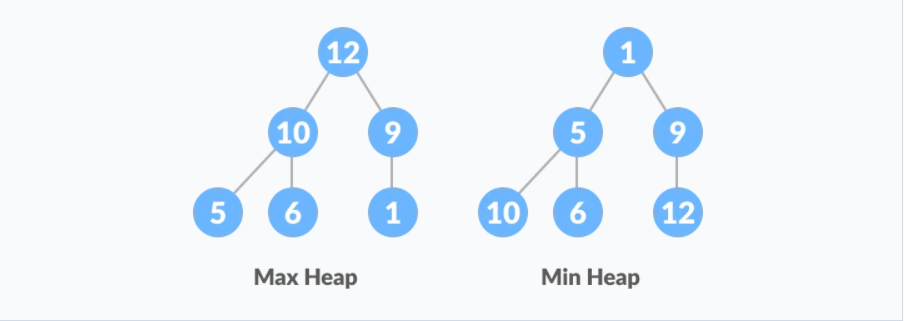
\includegraphics[scale=0.75]{heap}
\end{center}
\caption{Max-heap and min-heap. Source: \cite{heap}}
\end{figure}
\subsubsection{Build a min-heap}
To build a min heap, we: \cite{heapbuild}
\begin{itemize}
\item Create a new child node at the end of the heap (last level).
\item Add the new key to that node (append it to the array).
\item Move the child up until we reach the root node and the heap property is satisfied.
\end{itemize}
To remove/delete a root node in a min heap, we: \cite{heapbuild}
\begin{itemize}
\item Delete the root node.
\item Move the key of last child to root.
\item Compare the parent node with its children.
\item If the value of the parent is greater than its children, swap them, and repeat until the heap property is satisfied.
\end{itemize}
\subsubsection{Build a max-heap}
Building a max-heap is similar to building a min-heap.
\subsubsection{Pseudocodes}
\lstset{language=Pascal} 
\begin{lstlisting}
heapify(a[1..n], i)
begin
	max = i;
	left = 2 * i;
	right = 2 * i + 1;
	if (left <= n and a[left] > a[max]) then  max = left;
	if (right <= n and a[right] > a[max]) then max = right;
	if (max != i) then 
		begin
		swap(a[i], a[max]);
		heapify(a, n, max);
		end
end

heapsort(a[1..n])
begin
	for i := n div 2 - 1 downto 1 do heapify(a, i);
	for i := n downto 1 do 
		begin
		swap(a[0], a[i];
		heapify(a[1..i], 0)
		end
end
\end{lstlisting}
\textbf{Time complexity:} \cite{heap}
\begin{itemize}
\item Worst case: $O \left( {n \log n} \right).$
\item Best case: $O \left( {n \log n} \right).$
\item Average case: $O \left( {n \log n} \right).$
\end{itemize}
\textbf{Space complexity:} $O \left( {1} \right).$ \cite{heap}

\subsection{Merge sort}
Merge sort is a divide-and-conquer algorithm that was invented by John von Neumann in 1945. This is one of the most popular sorting algorithms. \\
\textbf{Ideas:} 
\begin{itemize}
\item Divide the array into two subarrays at the middle position.
\item Try to sort both subarrays, if we have not reached the base case yet, continue to divide them into subarrays.
\item Merge the sorted subarrays.
\end{itemize}
\textbf{Pseudocodes:}
\lstset{language=Pascal} 
\begin{lstlisting}
mergeSort(a[1..n])
begin
	if (n <= 1) do return;
	mid := n div 2;
	left[1..mid] := a[1..mid];
	right[1..n - mid] := a[mid + 1..n];
	
	mergeSort(left[1..mid]);
	mergeSort(right[1..n - mid]);
	
	i := 1; j := 1; k := 1;
	while (i <= mid and j <= n - mid)
		begin
		if (left[i] < right[j]) do 
			begin 
			a[k] := left[i];
			k := k + 1;
			i := i + 1;
			end 
		else 
			begin
			a[k] := right[j];
			k := k + 1;
			j := j + 1;
			end
	while (i <= mid) do
		begin
		a[k] := left[i];
		k := k + 1;
		i := i + 1;	
		end
	while (j <= n - mid) do
		begin
		a[k] := right[j];
		k := k + 1;
		j := j + 1;
		end
end
\end{lstlisting}
\textbf{Time complexity:}  \cite{merge}
\begin{itemize}
\item Worst case: $O \left( {n \log n} \right).$
\item Best case: $O \left( {n \log n} \right).$
\item Average case: $O \left( {n \log n} \right).$
\end{itemize}
\textbf{Space complexity:} $O \left( {n} \right).$ \cite{merge}

\newpage
\begin{thebibliography}{9}
\bibitem{gtvlt}
Le Minh Hoang (2002) \emph{Giai thuat va lap trinh}, Ha Noi University of Education Press

\bibitem{thayP}
Lectures from Dr. Nguyen Thanh Phuong

\bibitem{sscomp}
\url{https://iq.opengenus.org/time-complexity-of-selection-sort/}

\bibitem{comp}
\url{https://www.geeksforgeeks.org/analysis-of-different-sorting-techniques}

\bibitem{bubble}
\url{https://www.geeksforgeeks.org/bubble-sort/}

\bibitem{shaker}
\url{https://www.javatpoint.com/cocktail-sort}

\bibitem{shaksort}
\url{https://www.geeksforgeeks.org/cocktail-sort/}

\bibitem{shell}
\url{https://www.tutorialspoint.com/Shell-Sort}

\bibitem{heap}
\url{https://www.programiz.com/dsa/heap-sort}

\bibitem{heapbuild}
\url{https://www.educative.io/blog/data-structure-heaps-guide}

\bibitem{merge}
\url{https://www.programiz.com/dsa/merge-sort}

\end{thebibliography}
\end{document}